%!TEX root = ../report.tex

\chapter{Introduction}
\newcommand{\chapquote}[3]{\begin{quotation} \textit{#1} \end{quotation} \begin{flushright} - #2\end{flushright} }

\chapquote{``You can't cross the sea merely by standing and staring at the water.``}{Rabindranath Tagore}

More than two thirds of the earth surface is covered by ocean and other water bodies. For a human it is often impossible to be able to explore it extensively. 
For finding new source of energy, monitoring tsunami, global warming or may be just to learn about deep sea eco-system or may be to look for a lost ship or an airplane, the need for venturing into potentially dangerous 
underwater scenarios appears regularly, in fact getting more frequent. That's why more and more robots are being deployed in underwater scenarios and lot of research is going in this direction. 
Some of the exploration or monitoring tasks requires the robot to see underwater, in order to make intelligent decisions.
But underwater environment is very difficult for optical cameras, as light is attenuated and absorbed by the particles in the water. And lot of real life monitoring and mapping 
tasks take place in cluttered and turbid underwater scenario. The limited visibility range of optical sensor is a big challenge. Hence sonar is more practical choice for underwater sensing as the sound can travel 
long distances with comparatively little attenuation. Though there are challenges with acoustic sensing as well, for example, it has low signal-to-noise ratio, lower resolution and unwanted reflections also cause problems. \\

Patch matching is one of the fundamental tasks in todays myriad computer vision and image processing applications. Patch matching can be used as low-level tasks like image stitching \cite{brown2007automatic}, 
deriving structure from motion \cite{molton2004locally} or high-level task as object instance recognition \cite{lowe1999object}, object classification \cite{yao2012codebook}, multi-view reconstruction \cite{seitz2006comparison}, 
image-retrieval etc. 
Patch matching for acoustic images are getting increasingly useful in underwater scenarios for data association in simultaneous localization and mapping (SLAM), object tracking, sonar image mosaicing \cite{hurtos2012fourier}
etc. applications. Typical challenges in patch matching tasks are different viewing points, variations in illumination of the scene, occlusions and different sensor settings. For patch matching in sonar images the typical issues 
with sonar images adds to the overall challenge, for example low signal to noise ratio, less of visibility causes the underlying object features to be not so prominent as a normal image. So it has been found that it is very 
challenging task to manually design features for the matching task is very challenging. %TODO add source Also the popular hand designed features such as SIFT \cite{lowe2004distinctive} are not always very effective in sonar images.

\section{Motivation}

In Valdenegro et al. \cite{stateoftheart} it was first displayed that deep learning methods can be directly applied to the sonar image patch classification task, without use of any hand designed features it is still possible 
to perform a patch matching task with high accuracy. In \cite{stateoftheart} the authors recorded forward looking sonar images of different objects in underwater environment and generated balanced dataset
of image patches for the classification task.
Two channel convolutional network and Siamese convolutional network were used in predicting the binary classification scores (table \ref{best_results_stateoftheart}) on unseen test data. Using Two channel CNN the overall 
best result obtained was of roc area under curve of 0.894, with test accuracy of 82.9\%. The reported results are
better than both classic keypoint matching methods (AUC 0.61 to 0.68) and ML-based methods such as Support Vector Machine (SVM) and Random Forests (AUC 0.65 to 0.80). These findings were pivotal for the work presented in this thesis.

\begin{table}
\centering
 \begin{tabular}{|c c c c c|} 
 \hline\hline
 Network Type & Output & Test Objects & AUC & Mean Accuracy \\ [0.5ex] 
 \hline
 2-Chan CNN & Score & Different & 0.894 & 82.9\% \\ 
 \hline
 Siamese CNN & Score & Different & 0.826 & 77.0\% \\
 \hline \hline
\end{tabular}
\caption{Best result from Valdenegro et. al. 'Different' represents the underlying test objects were different from the train objects. The binary prediction scores are presented here from the original 
results in \cite{stateoftheart}}
\label{best_results_stateoftheart}
\end{table}

\newpage

\section{Problem Statement}
However the results in \cite{stateoftheart} is far from perfect yet and the mis-classifications affect the object detection, recognition and tracking, 
which are dependent on the patch matching task. It is desired that the result is further improved. With this goal the same dataset has been obtained from the \cite{stateoftheart} for further evaluation.
In this thesis more advanced architectures (such as Densenet) \cite{densenet} will be evaluated on the data and the goal is to improve the state of the art on the dataset. 

%\flushbottom
%\newpage

\begin{wrapfigure}[18]{l}{6.5cm}
\hspace{1cm}
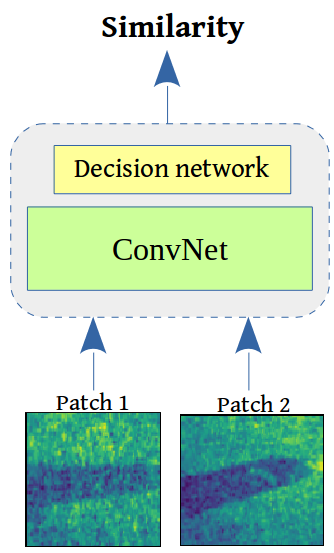
\includegraphics[width=4cm]{images/densenet/similarity_fn}
\caption{Use of convolutional network for learning general similarity function for image patches. The patches in the image are samples taken from the data used in this thesis. 
Inspired from Zagoruyko et al.\cite{zagoruyko2015learning}}
\label{similarity_function_wraped}
\end{wrapfigure} 

For performing the patch matching task without using any hand designed features such as SIFT \cite{lowe2004distinctive}, we need to encode a network to learn the general
similarity function (figure \ref{similarity_function_wraped})
for sonar image patches. Which is able to predict that two input sonar patches contain different views of a same object or not i.e matching or non-matching respectively.

With the goal of obtaining the best possible result in the evaluation, best hyperparameter search needs to be 
performed for each of the networks. The hyperparameters are the parameters of network or learning process whose values are already set before the training starts \cite{wikihyper}. For example the starting learning rate 
or the optimizer can be fixed before the training process start. 

Performing best hyper parameter search for each of the architectures is very important part of the evaluation. Another objective of this work is to do a comparative analysis of the performance of all the architectures.

%\subsection{Similarity function}





%\subsection{...}


%\subsection{...}
